% $Author: oscar $
% $Date: 2009-09-15 16:53:48 +0200 (Tue, 15 Sep 2009) $
% $Revision: 29111 $
%=================================================================
\ifx\wholebook\relax\else
% --------------------------------------------
% Lulu:
	\documentclass[a4paper,10pt,twoside]{book}
	\usepackage[
		papersize={6.13in,9.21in},
		hmargin={.815in,.815in},
		vmargin={.98in,.98in},
		ignoreheadfoot
	]{geometry}
  \usepackage[hangul]{kotex}
	% $Author: oscar $
% $Date: 2009-09-13 20:58:29 +0200 (Sun, 13 Sep 2009) $
% $Revision: 29070 $
%=============================================================
% NB: documentclass must be set in main document.
% Allows book to be generated in multiple formats.
%=============================================================
%:Packages
\usepackage[T1]{fontenc}  %%%%%really important to get the code directly in the text!
\usepackage{palatino}
\usepackage{ifthen}
\usepackage{graphicx}
\graphicspath{{figures/}}
\usepackage{xspace}
\usepackage{makeidx}
\usepackage{isodateo} % enable \isodate
\usepackage{amssymb,textcomp}
%=============================================================
%:More packages
%\usepackage[english]{babel}
%\usepackage{lmodern}
%\usepackage[scaled=0.85]{helvet}
%\usepackage{microtype}
%\usepackage{theorem}
%\usepackage{float}
%\usepackage{longtable}
%\usepackage[nottoc]{tocbibind}
%\usepackage{multicol}
%\usepackage{booktabs}	% book-style tables
%\usepackage{topcapt}	% enables \topcaption
%\usepackage{multirow}
%\usepackage{tabularx}
%\usepackage{alltt}
\usepackage[usenames,dvipsnames]{color}
%\usepackage[hang]{subfigure}\makeatletter\def\p@subfigure{\thefigure\,}\makeatother
%\usepackage{rotating}
%\usepackage{enumitem}	% apb: allows more control over tags in enumerations
%\usepackage{verbatim}     % for comment environment
%\usepackage{varioref}	% for page references that work
%\usepackage{needspace}
%\usepackage[newparttoc]{titlesec}
%\usepackage{titletoc}
%\usepackage{wrapfig}
\usepackage[
	colorlinks=true,
	linkcolor=black,
	urlcolor=black,
	citecolor=black
]{hyperref}   % should come last
%=============================================================
%:URL style
\makeatletter
\def\url@leostyle{%
  \@ifundefined{selectfont}{\def\UrlFont{\sf}}{\def\UrlFont{\sffamily}}}
\makeatother
\urlstyle{leo}
%=============================================================
%:Booleans
\newboolean{lulu}
\setboolean{lulu}{false}
\newcommand{\ifluluelse}[2]{\ifthenelse{\boolean{lulu}}{#1}{#2}}
%=============================================================
%:Editorial comment macros
\newcommand{\nnbb}[2]{
  \fbox{\bfseries\sffamily\scriptsize#1}
  {\sf\small$\blacktriangleright$\textit{#2}$\blacktriangleleft$}
}
\newcommand{\on}[1]{\nnbb{Oscar}{#1}}
\newcommand{\here}{\nnbb{CONTINUE}{HERE}}
%=============================================================
%:Abbreviation macros
\newcommand{\ie}{\emph{i.e.},\xspace}
\newcommand{\eg}{\emph{e.g.},\xspace}
\newcommand{\etc}{\emph{etc.}\xspace}
\newcommand{\etal}{\emph{et al.}\xspace}
\newcommand{\straightquote}{"}
\newcommand{\sba}{\url{SquareBracketAssociates.org}\xspace}
%=============================================================
%:Patterns
% \newcommand{\pattern}[2]{\newpage\section{{\sf #1}}\label{pat:#2}}
% \newcommand{\pattern}[2]{\newpage\index{#1 (Pattern)}\section{#1}\label{pat:#2}}
\newcommand{\pattern}[2]{\cleardoublepage\index{#1 (패턴)}\section{#1}\label{pat:#2}}
\newcommand{\thumbnail}[2]{\index{#1 (패턴)}\subsection{#1}\label{pat:#2}}
\newcommand{\thumblang}[2]{\index{#1 (패턴 랭귀지)}\subsection{#1}\label{pat:#2}}
\newcommand{\variant}[1]{{\emph{#1}}\xspace}
% \newcommand{\problem}[1]{\subsection*{Problem}\emph{#1}}
\newcommand{\intent}[1]{\paragraph{의도}\emph{#1}}
\newcommand{\problem}[1]{\paragraph{문제}\emph{#1}}
\newcommand{\solution}[1]{\paragraph{해결}\emph{#1}}
\newcommand{\discussion}[0]{\paragraph{토론}}
\newcommand{\cmd}[1]{{\tt #1}\xspace}
%=============================================================
%:Environments
\newenvironment{bulletlist}{\begin{itemize}\setlength{\itemsep}{0ex}}
{\end{itemize}}
%=============================================================
%:Cross reference macros
\newcommand{\chalabel}[1]{\label{cha:#1}}
\newcommand{\seclabel}[1]{\label{sec:#1}}
\newcommand{\figlabel}[1]{\label{fig:#1}}
\newcommand{\tablabel}[1]{\label{tab:#1}}
\newcommand{\rulelabel}[1]{\label{rule:#1}}
\newcommand{\eglabel}[1]{\label{eg:#1}}
\newcommand{\scrlabel}[1]{\label{scr:#1}}
\newcommand{\mthlabel}[1]{\label{mth:#1}}
\newcommand{\clslabel}[1]{\label{cls:#1}}
\newcommand{\faqlabel}[1]{\label{faq:#1}}
%\newcommand{\charef}[1]{Chapter~\ref{cha:#1}\xspace}
%\newcommand{\secref}[1]{Section~\ref{sec:#1}\xspace}
\newcommand{\figref}[1]{Figure~\ref{fig:#1}\xspace}
% \newcommand{\patpgref}[2]{\hyperref[pat:#2]{\sf #1} [p.~\pageref{pat:#2}]\xspace}
\newcommand{\patpgref}[2]{\index{#1 (Pattern)}\hyperref[pat:#2]{#1} [p.~\pageref{pat:#2}]\xspace}
\newcommand{\patlangpgref}[2]{\index{#1 (Pattern language)}\hyperref[pat:#2]{#1} [p.~\pageref{pat:#2}]\xspace}
% \newcommand{\patref}[2]{\hyperref[pat:#2]{\sf #1}\xspace}
\newcommand{\patref}[2]{\index{#1 (Pattern)}\hyperref[pat:#2]{#1}\xspace}
\newcommand{\patlangref}[2]{\index{#1 (Pattern language)}\hyperref[pat:#2]{#1}\xspace}
% \newcommand{\charef}[2]{\hyperref[cha:#2]{\underline{\sf #1}}\xspace}
% \newcommand{\charef}[2]{\hyperref[cha:#2]{\sf #1}\xspace}
\newcommand{\charef}[2]{\index{#1 (Pattern cluster)}\hyperref[cha:#2]{#1}\xspace}
% \newcommand{\chapgref}[2]{\hyperref[cha:#2]{\sf #1} [p.~\pageref{cha:#2}]\xspace}
\newcommand{\chapgref}[2]{\index{#1 (Pattern cluster)}\hyperref[cha:#2]{#1} [p.~\pageref{cha:#2}]\xspace}
%\newcommand{\Figref}[1]{Figure~\ref{fig:#1}\xspace}
%\newcommand{\appref}[1]{Appendix~\ref{app:#1}\xspace}
%\newcommand{\tabref}[1]{Table~\ref{tab:#1}\xspace}
%\newcommand{\ruleref}[1]{\ref{rule:#1}\xspace}
%\newcommand{\egref}[1]{example~\ref{eg:#1}\xspace}
%\newcommand{\Egref}[1]{Example~\ref{eg:#1}\xspace}
%\newcommand{\scrref}[1]{script~\ref{scr:#1}\xspace}
%\newcommand{\Scrref}[1]{Script~\ref{scr:#1}\xspace}
%\newcommand{\tscrref}[1]{the script~\ref{scr:#1}\xspace}
%\newcommand{\Tscrref}[1]{The script~\ref{scr:#1}\xspace}
%\newcommand{\mthref}[1]{method~\ref{mth:#1}\xspace}
%\newcommand{\mthsref}[1]{methods~\ref{mth:#1}\xspace}
%\newcommand{\Mthref}[1]{Method~\ref{mth:#1}\xspace}
%\newcommand{\tmthref}[1]{the method~\ref{mth:#1}\xspace}
%\newcommand{\Tmthref}[1]{The method~\ref{mth:#1}\xspace}
%\newcommand{\clsref}[1]{class~\ref{cls:#1}\xspace}
%\newcommand{\tclsref}[1]{the class~\ref{cls:#1}\xspace}
%\newcommand{\Tclsref}[1]{The class~\ref{cls:#1}\xspace}
%=============================================================
%:Page Layout
\setlength{\headsep}{1cm}
%=============================================================
%:Menu item macro
%\definecolor{lightgray}{gray}{0.89}
%\newcommand{\menu}[1]{{%
%	\setlength{\fboxsep}{0pt}%
%	\colorbox{lightgray}{{{\upshape\sffamily\strut \,#1\,}}}}}
%\newcommand{\go}{\,$\triangleright$\,}
%\newcommand{\short}[1]{\mbox{{\sc cmd}\hspace{0.08em}--\hspace{0.09em}#1}\xspace}
%\newcommand{\button}[1]{{%
%	\setlength{\fboxsep}{0pt}%
%	\fbox{{\upshape\sffamily\strut \,#1\,}}}}
%\newcommand{\toolsflap}{\textit{Tools} flap\xspace}
%=============================================================
%:Section depth
%\setcounter{secnumdepth}{2}
%
%\DeclareGraphicsExtensions{.pdf, .jpg, .png}
%=============================================================
%:PDF setup
\hypersetup{
   pdftitle={Object-Oriented Reengineering Patterns},
   pdfauthor={Serge Demeyer, St\'ephane Ducasse, Oscar Nierstrasz},
   pdfkeywords={Reengineering, Object-Oriented Programming, Patterns},
   pdfsubject={Computer Science}
}
%=============================================================
%:Page layout and appearance
%\renewcommand{\chaptermark}[1]{\markboth{#1}{}}
%\renewcommand{\sectionmark}[1]{\markright{\thesection\ #1}}
%\renewpagestyle{plain}[\small\itshape]{%
%	\setheadrule{0pt}%
%	\sethead[][][]{}{}{}%
%	\setfoot[][][]{}{}{}}
%\renewpagestyle{headings}[\small\itshape]{%
%	\setheadrule{0pt}%
%	\setmarks{chapter}{section}%
%	\sethead[\thepage][][\chaptertitle]{\sectiontitle}{}{\thepage}%
%	\setfoot[][][]{}{}{}}
%=============================================================
%:Title section setup and TOC numbering depth
%\setcounter{secnumdepth}{1}
%\setcounter{tocdepth}{1}
%\titleformat{\part}[display]{\centering}{\huge\partname\ \thepart}{1em}{\Huge\textbf}[]
%\titleformat{\chapter}[display]{}{\huge\chaptertitlename\ \thechapter}{1em}{\Huge\raggedright\textbf}[]
%\titlecontents{part}[3pc]{%
%		\pagebreak[2]\addvspace{1em plus.4em minus.2em}%
%		\leavevmode\large\bfseries}
%	{\contentslabel{3pc}}{\hspace*{-3pc}}
%	{}[\nopagebreak]
%\titlecontents{chapter}[3pc]{%
%		\pagebreak[0]\addvspace{1em plus.2em minus.2em}%
%		\leavevmode\bfseries}
%	{\contentslabel{3pc}}{}
%	{\hfill\contentspage}[\nopagebreak]
%\dottedcontents{section}[3pc]{}{3pc}{1pc}
%\dottedcontents{subsection}[3pc]{}{0pc}{1pc}
%\let\origdoublepage\cleardoublepage
%\newcommand{\clearemptydoublepage}{%
%  \clearpage
%  {\pagestyle{empty}\origdoublepage}}
%\let\cleardoublepage\clearemptydoublepage % see http://www.tex.ac.uk/cgi-bin/texfaq2html?label=patch
%=============================================================
%:Listings package configuration
\newcommand{\caret}{\makebox{\raisebox{0.4ex}{\footnotesize{$\wedge$}}}}
% \newcommand{\escape}{{\sf \textbackslash}}
\definecolor{source}{gray}{0.95}
\usepackage{listings}
\lstdefinelanguage{Smalltalk}{
  morestring=[d]',
% Adapt this to other languages!
%  morecomment=[s]{"}{"},
  alsoletter={\#:},
  %escapechar={!},
  literate=
    {BANG}{!}1
%    {UNDERSCORE}{\_}1
    {\\st}{Smalltalk}9 % convenience -- in case \st occurs in code
    % {'}{{\textquotesingle}}1 % replaced by upquote=true in \lstset
%    {_}{{$\leftarrow$}}1
    {>>>}{{\sep}}1
    {^}{{$\uparrow$}}1
    {~}{{$\sim$}}1
    {-}{{\sf -\hspace{-0.13em}-}}1  % the goal is to make - the same width as +
    {+}{\raisebox{0.08ex}{+}}1		% and to raise + off the baseline to match -
    {-->}{{\quad$\longrightarrow$\quad}}3
	, % Don't forget the comma at the end!
  tabsize=4
}[keywords,comments,strings]

\lstset{language=Smalltalk,
	basicstyle=\sffamily,
	keywordstyle=\color{black}\bfseries,
	% stringstyle=\ttfamily, % Ugly! do we really want this? -- on
	mathescape=true,
	showstringspaces=false,
	keepspaces=true,
	breaklines=true,
	breakautoindent=true,
	backgroundcolor=\color{source},
	lineskip={-1pt}, % Ugly hack
	upquote=true, % straight quote; requires textcomp package
	columns=fullflexible} % no fixed width fonts
% \newcommand{\ct}{\lstinline[mathescape=false,basicstyle={\sffamily\upshape}]}
\newcommand{\ct}{\lstinline[mathescape=false,backgroundcolor=\color{white},basicstyle={\sffamily\upshape}]}
\newcommand{\lct}[1]{{\textsf{\textup{#1}}}}
%\newcommand{\scat}[1]{\emph{\textsf{#1}}\xspace}
%\newcommand{\prot}[1]{\emph{\textsf{#1}}\xspace}
% NB: No argument!
\lstnewenvironment{code}[0]{%
	\lstset{%
		% frame=lines,
		frame=single,
		framerule=0pt,
		mathescape=false
	}
}{}
%\def\ignoredollar#1{}
%=============================================================
%:Reserving space
%\newcommand{\needlines}[1]{\Needspace{#1\baselineskip}}
%=============================================================
%:Indexing macros
% Macros ending with "ind" generate text as well as an index entry
% Macros ending with "index" *only* generate an index entry
\newcommand{\ind}[1]{\index{#1}#1\xspace} % plain text
\newcommand{\subind}[2]{\index{#1!#2}#2\xspace} % show #2, subindex under #1
\newcommand{\emphind}[1]{\index{#1}\emph{#1}\xspace} % emph #1
\newcommand{\emphsubind}[2]{\index{#1!#2}\emph{#2}\xspace} % show emph #2, subindex under #1
\newcommand{\patind}[1]{\index{#1@#1 (pattern)}\ct{#1}\xspace} % pattern
\newcommand{\seeindex}[2]{\index{#1|see{#2}}} % #1, see #2
%\newcommand{\boldidx}[1]{{\bf #1}} % breaks hyperlink
%\newcommand{\indmain}[1]{\index{#1}#1\xspace} 
%\newcommand{\emphsubindmain}[2]{\index{#1!#2}\emph{#2}\xspace} % subindex, main entry
%\newcommand{\subindmain}[2]{\index{#1!#2}#2\xspace} % subindex, main entry
%\newcommand{\clsindmain}[1]{\index{#1!\#@(class)}\ct{#1}\xspace} % class main
%\newcommand{\indexmain}[1]{\index{#1}} 
%=============================================================
\parskip 1ex
%=============================================================

	\pagestyle{headings}
	\setboolean{lulu}{true}
% --------------------------------------------
% A4:
%	\documentclass[a4paper,11pt,twoside]{book}
%	% $Author: oscar $
% $Date: 2009-09-13 20:58:29 +0200 (Sun, 13 Sep 2009) $
% $Revision: 29070 $
%=============================================================
% NB: documentclass must be set in main document.
% Allows book to be generated in multiple formats.
%=============================================================
%:Packages
\usepackage[T1]{fontenc}  %%%%%really important to get the code directly in the text!
\usepackage{palatino}
\usepackage{ifthen}
\usepackage{graphicx}
\graphicspath{{figures/}}
\usepackage{xspace}
\usepackage{makeidx}
\usepackage{isodateo} % enable \isodate
\usepackage{amssymb,textcomp}
%=============================================================
%:More packages
%\usepackage[english]{babel}
%\usepackage{lmodern}
%\usepackage[scaled=0.85]{helvet}
%\usepackage{microtype}
%\usepackage{theorem}
%\usepackage{float}
%\usepackage{longtable}
%\usepackage[nottoc]{tocbibind}
%\usepackage{multicol}
%\usepackage{booktabs}	% book-style tables
%\usepackage{topcapt}	% enables \topcaption
%\usepackage{multirow}
%\usepackage{tabularx}
%\usepackage{alltt}
\usepackage[usenames,dvipsnames]{color}
%\usepackage[hang]{subfigure}\makeatletter\def\p@subfigure{\thefigure\,}\makeatother
%\usepackage{rotating}
%\usepackage{enumitem}	% apb: allows more control over tags in enumerations
%\usepackage{verbatim}     % for comment environment
%\usepackage{varioref}	% for page references that work
%\usepackage{needspace}
%\usepackage[newparttoc]{titlesec}
%\usepackage{titletoc}
%\usepackage{wrapfig}
\usepackage[
	colorlinks=true,
	linkcolor=black,
	urlcolor=black,
	citecolor=black
]{hyperref}   % should come last
%=============================================================
%:URL style
\makeatletter
\def\url@leostyle{%
  \@ifundefined{selectfont}{\def\UrlFont{\sf}}{\def\UrlFont{\sffamily}}}
\makeatother
\urlstyle{leo}
%=============================================================
%:Booleans
\newboolean{lulu}
\setboolean{lulu}{false}
\newcommand{\ifluluelse}[2]{\ifthenelse{\boolean{lulu}}{#1}{#2}}
%=============================================================
%:Editorial comment macros
\newcommand{\nnbb}[2]{
  \fbox{\bfseries\sffamily\scriptsize#1}
  {\sf\small$\blacktriangleright$\textit{#2}$\blacktriangleleft$}
}
\newcommand{\on}[1]{\nnbb{Oscar}{#1}}
\newcommand{\here}{\nnbb{CONTINUE}{HERE}}
%=============================================================
%:Abbreviation macros
\newcommand{\ie}{\emph{i.e.},\xspace}
\newcommand{\eg}{\emph{e.g.},\xspace}
\newcommand{\etc}{\emph{etc.}\xspace}
\newcommand{\etal}{\emph{et al.}\xspace}
\newcommand{\straightquote}{"}
\newcommand{\sba}{\url{SquareBracketAssociates.org}\xspace}
%=============================================================
%:Patterns
% \newcommand{\pattern}[2]{\newpage\section{{\sf #1}}\label{pat:#2}}
% \newcommand{\pattern}[2]{\newpage\index{#1 (Pattern)}\section{#1}\label{pat:#2}}
\newcommand{\pattern}[2]{\cleardoublepage\index{#1 (패턴)}\section{#1}\label{pat:#2}}
\newcommand{\thumbnail}[2]{\index{#1 (패턴)}\subsection{#1}\label{pat:#2}}
\newcommand{\thumblang}[2]{\index{#1 (패턴 랭귀지)}\subsection{#1}\label{pat:#2}}
\newcommand{\variant}[1]{{\emph{#1}}\xspace}
% \newcommand{\problem}[1]{\subsection*{Problem}\emph{#1}}
\newcommand{\intent}[1]{\paragraph{의도}\emph{#1}}
\newcommand{\problem}[1]{\paragraph{문제}\emph{#1}}
\newcommand{\solution}[1]{\paragraph{해결}\emph{#1}}
\newcommand{\discussion}[0]{\paragraph{토론}}
\newcommand{\cmd}[1]{{\tt #1}\xspace}
%=============================================================
%:Environments
\newenvironment{bulletlist}{\begin{itemize}\setlength{\itemsep}{0ex}}
{\end{itemize}}
%=============================================================
%:Cross reference macros
\newcommand{\chalabel}[1]{\label{cha:#1}}
\newcommand{\seclabel}[1]{\label{sec:#1}}
\newcommand{\figlabel}[1]{\label{fig:#1}}
\newcommand{\tablabel}[1]{\label{tab:#1}}
\newcommand{\rulelabel}[1]{\label{rule:#1}}
\newcommand{\eglabel}[1]{\label{eg:#1}}
\newcommand{\scrlabel}[1]{\label{scr:#1}}
\newcommand{\mthlabel}[1]{\label{mth:#1}}
\newcommand{\clslabel}[1]{\label{cls:#1}}
\newcommand{\faqlabel}[1]{\label{faq:#1}}
%\newcommand{\charef}[1]{Chapter~\ref{cha:#1}\xspace}
%\newcommand{\secref}[1]{Section~\ref{sec:#1}\xspace}
\newcommand{\figref}[1]{Figure~\ref{fig:#1}\xspace}
% \newcommand{\patpgref}[2]{\hyperref[pat:#2]{\sf #1} [p.~\pageref{pat:#2}]\xspace}
\newcommand{\patpgref}[2]{\index{#1 (Pattern)}\hyperref[pat:#2]{#1} [p.~\pageref{pat:#2}]\xspace}
\newcommand{\patlangpgref}[2]{\index{#1 (Pattern language)}\hyperref[pat:#2]{#1} [p.~\pageref{pat:#2}]\xspace}
% \newcommand{\patref}[2]{\hyperref[pat:#2]{\sf #1}\xspace}
\newcommand{\patref}[2]{\index{#1 (Pattern)}\hyperref[pat:#2]{#1}\xspace}
\newcommand{\patlangref}[2]{\index{#1 (Pattern language)}\hyperref[pat:#2]{#1}\xspace}
% \newcommand{\charef}[2]{\hyperref[cha:#2]{\underline{\sf #1}}\xspace}
% \newcommand{\charef}[2]{\hyperref[cha:#2]{\sf #1}\xspace}
\newcommand{\charef}[2]{\index{#1 (Pattern cluster)}\hyperref[cha:#2]{#1}\xspace}
% \newcommand{\chapgref}[2]{\hyperref[cha:#2]{\sf #1} [p.~\pageref{cha:#2}]\xspace}
\newcommand{\chapgref}[2]{\index{#1 (Pattern cluster)}\hyperref[cha:#2]{#1} [p.~\pageref{cha:#2}]\xspace}
%\newcommand{\Figref}[1]{Figure~\ref{fig:#1}\xspace}
%\newcommand{\appref}[1]{Appendix~\ref{app:#1}\xspace}
%\newcommand{\tabref}[1]{Table~\ref{tab:#1}\xspace}
%\newcommand{\ruleref}[1]{\ref{rule:#1}\xspace}
%\newcommand{\egref}[1]{example~\ref{eg:#1}\xspace}
%\newcommand{\Egref}[1]{Example~\ref{eg:#1}\xspace}
%\newcommand{\scrref}[1]{script~\ref{scr:#1}\xspace}
%\newcommand{\Scrref}[1]{Script~\ref{scr:#1}\xspace}
%\newcommand{\tscrref}[1]{the script~\ref{scr:#1}\xspace}
%\newcommand{\Tscrref}[1]{The script~\ref{scr:#1}\xspace}
%\newcommand{\mthref}[1]{method~\ref{mth:#1}\xspace}
%\newcommand{\mthsref}[1]{methods~\ref{mth:#1}\xspace}
%\newcommand{\Mthref}[1]{Method~\ref{mth:#1}\xspace}
%\newcommand{\tmthref}[1]{the method~\ref{mth:#1}\xspace}
%\newcommand{\Tmthref}[1]{The method~\ref{mth:#1}\xspace}
%\newcommand{\clsref}[1]{class~\ref{cls:#1}\xspace}
%\newcommand{\tclsref}[1]{the class~\ref{cls:#1}\xspace}
%\newcommand{\Tclsref}[1]{The class~\ref{cls:#1}\xspace}
%=============================================================
%:Page Layout
\setlength{\headsep}{1cm}
%=============================================================
%:Menu item macro
%\definecolor{lightgray}{gray}{0.89}
%\newcommand{\menu}[1]{{%
%	\setlength{\fboxsep}{0pt}%
%	\colorbox{lightgray}{{{\upshape\sffamily\strut \,#1\,}}}}}
%\newcommand{\go}{\,$\triangleright$\,}
%\newcommand{\short}[1]{\mbox{{\sc cmd}\hspace{0.08em}--\hspace{0.09em}#1}\xspace}
%\newcommand{\button}[1]{{%
%	\setlength{\fboxsep}{0pt}%
%	\fbox{{\upshape\sffamily\strut \,#1\,}}}}
%\newcommand{\toolsflap}{\textit{Tools} flap\xspace}
%=============================================================
%:Section depth
%\setcounter{secnumdepth}{2}
%
%\DeclareGraphicsExtensions{.pdf, .jpg, .png}
%=============================================================
%:PDF setup
\hypersetup{
   pdftitle={Object-Oriented Reengineering Patterns},
   pdfauthor={Serge Demeyer, St\'ephane Ducasse, Oscar Nierstrasz},
   pdfkeywords={Reengineering, Object-Oriented Programming, Patterns},
   pdfsubject={Computer Science}
}
%=============================================================
%:Page layout and appearance
%\renewcommand{\chaptermark}[1]{\markboth{#1}{}}
%\renewcommand{\sectionmark}[1]{\markright{\thesection\ #1}}
%\renewpagestyle{plain}[\small\itshape]{%
%	\setheadrule{0pt}%
%	\sethead[][][]{}{}{}%
%	\setfoot[][][]{}{}{}}
%\renewpagestyle{headings}[\small\itshape]{%
%	\setheadrule{0pt}%
%	\setmarks{chapter}{section}%
%	\sethead[\thepage][][\chaptertitle]{\sectiontitle}{}{\thepage}%
%	\setfoot[][][]{}{}{}}
%=============================================================
%:Title section setup and TOC numbering depth
%\setcounter{secnumdepth}{1}
%\setcounter{tocdepth}{1}
%\titleformat{\part}[display]{\centering}{\huge\partname\ \thepart}{1em}{\Huge\textbf}[]
%\titleformat{\chapter}[display]{}{\huge\chaptertitlename\ \thechapter}{1em}{\Huge\raggedright\textbf}[]
%\titlecontents{part}[3pc]{%
%		\pagebreak[2]\addvspace{1em plus.4em minus.2em}%
%		\leavevmode\large\bfseries}
%	{\contentslabel{3pc}}{\hspace*{-3pc}}
%	{}[\nopagebreak]
%\titlecontents{chapter}[3pc]{%
%		\pagebreak[0]\addvspace{1em plus.2em minus.2em}%
%		\leavevmode\bfseries}
%	{\contentslabel{3pc}}{}
%	{\hfill\contentspage}[\nopagebreak]
%\dottedcontents{section}[3pc]{}{3pc}{1pc}
%\dottedcontents{subsection}[3pc]{}{0pc}{1pc}
%\let\origdoublepage\cleardoublepage
%\newcommand{\clearemptydoublepage}{%
%  \clearpage
%  {\pagestyle{empty}\origdoublepage}}
%\let\cleardoublepage\clearemptydoublepage % see http://www.tex.ac.uk/cgi-bin/texfaq2html?label=patch
%=============================================================
%:Listings package configuration
\newcommand{\caret}{\makebox{\raisebox{0.4ex}{\footnotesize{$\wedge$}}}}
% \newcommand{\escape}{{\sf \textbackslash}}
\definecolor{source}{gray}{0.95}
\usepackage{listings}
\lstdefinelanguage{Smalltalk}{
  morestring=[d]',
% Adapt this to other languages!
%  morecomment=[s]{"}{"},
  alsoletter={\#:},
  %escapechar={!},
  literate=
    {BANG}{!}1
%    {UNDERSCORE}{\_}1
    {\\st}{Smalltalk}9 % convenience -- in case \st occurs in code
    % {'}{{\textquotesingle}}1 % replaced by upquote=true in \lstset
%    {_}{{$\leftarrow$}}1
    {>>>}{{\sep}}1
    {^}{{$\uparrow$}}1
    {~}{{$\sim$}}1
    {-}{{\sf -\hspace{-0.13em}-}}1  % the goal is to make - the same width as +
    {+}{\raisebox{0.08ex}{+}}1		% and to raise + off the baseline to match -
    {-->}{{\quad$\longrightarrow$\quad}}3
	, % Don't forget the comma at the end!
  tabsize=4
}[keywords,comments,strings]

\lstset{language=Smalltalk,
	basicstyle=\sffamily,
	keywordstyle=\color{black}\bfseries,
	% stringstyle=\ttfamily, % Ugly! do we really want this? -- on
	mathescape=true,
	showstringspaces=false,
	keepspaces=true,
	breaklines=true,
	breakautoindent=true,
	backgroundcolor=\color{source},
	lineskip={-1pt}, % Ugly hack
	upquote=true, % straight quote; requires textcomp package
	columns=fullflexible} % no fixed width fonts
% \newcommand{\ct}{\lstinline[mathescape=false,basicstyle={\sffamily\upshape}]}
\newcommand{\ct}{\lstinline[mathescape=false,backgroundcolor=\color{white},basicstyle={\sffamily\upshape}]}
\newcommand{\lct}[1]{{\textsf{\textup{#1}}}}
%\newcommand{\scat}[1]{\emph{\textsf{#1}}\xspace}
%\newcommand{\prot}[1]{\emph{\textsf{#1}}\xspace}
% NB: No argument!
\lstnewenvironment{code}[0]{%
	\lstset{%
		% frame=lines,
		frame=single,
		framerule=0pt,
		mathescape=false
	}
}{}
%\def\ignoredollar#1{}
%=============================================================
%:Reserving space
%\newcommand{\needlines}[1]{\Needspace{#1\baselineskip}}
%=============================================================
%:Indexing macros
% Macros ending with "ind" generate text as well as an index entry
% Macros ending with "index" *only* generate an index entry
\newcommand{\ind}[1]{\index{#1}#1\xspace} % plain text
\newcommand{\subind}[2]{\index{#1!#2}#2\xspace} % show #2, subindex under #1
\newcommand{\emphind}[1]{\index{#1}\emph{#1}\xspace} % emph #1
\newcommand{\emphsubind}[2]{\index{#1!#2}\emph{#2}\xspace} % show emph #2, subindex under #1
\newcommand{\patind}[1]{\index{#1@#1 (pattern)}\ct{#1}\xspace} % pattern
\newcommand{\seeindex}[2]{\index{#1|see{#2}}} % #1, see #2
%\newcommand{\boldidx}[1]{{\bf #1}} % breaks hyperlink
%\newcommand{\indmain}[1]{\index{#1}#1\xspace} 
%\newcommand{\emphsubindmain}[2]{\index{#1!#2}\emph{#2}\xspace} % subindex, main entry
%\newcommand{\subindmain}[2]{\index{#1!#2}#2\xspace} % subindex, main entry
%\newcommand{\clsindmain}[1]{\index{#1!\#@(class)}\ct{#1}\xspace} % class main
%\newcommand{\indexmain}[1]{\index{#1}} 
%=============================================================
\parskip 1ex
%=============================================================

%	\usepackage{a4wide}
% --------------------------------------------
	\begin{document}
	\renewcommand{\nnbb}[2]{} % Disable editorial comments
	\sloppy
\fi
%=================================================================
\chapter{방향 설정}
\chalabel{SettingDirection}

리엔지니어링 프로젝트를 시작하면 경영진, 사용자, 자신의 팀 등 다양한 측면에서 영향을 받는다. 기술적으로 가장 흥미로운 부분이나 가장 쉽게 고칠 수 있을 것 같은 부분에 집중하고 싶은 유혹에 빠지기 쉽다. 하지만 최선의 전략은 무엇일까? 리엔지니어링 작업의 방향을 어떻게 설정하고, 일단 시작한 후에는 어떻게 방향을 유지할까?

%-----------------------------------------------------------------
\subsection*{포스: 주요한 요구사항}
\begin{bulletlist}
  \item 일반적인 리엔지니어링 프로젝트에는 서로 다른 방향을 가지는 많은 이해관계가 얽혀 있다. 기술적, 인체공학적, 경제적, 정치적 고려 사항으로 인해 여러분과 여러분의 팀은 집중력을 확립하고 유지하기가 어려울 것이다. 

  \item 리엔지니어링 프로젝트의 커뮤니케이션은 기존 프로젝트의 개발팀의 유무에 따라 복잡해질 수 있다.

  \item 레거시 시스템은 시스템의 미래에 최선이 아닐 수 있는 특정 \ind{아키텍처(architecture)}로 사용자에게 강요할 수 있다.

  \item 레거시 소프트웨어에서 많은 문제를 발견할 수 있으며 우선순위를 설정하기가 어려울 것이다.

  \item 프로젝트에 가장 적합한 것이 아니라 가장 관심 있는 기술적 문제에 집중하는 유혹에 빠지기 쉽다.

  \item 레거시 시스템의 문제가 있는 구성 요소를 래핑(wrapping)할지, 리팩터링(refactoring)할지, 다시 작성(rewrite)할지 결정하기 어려울 수 있다. 이러한 각 옵션은 서로 다른 위험을 해결하며 필요한 노력, 결과를 평가할 수 있는 속도, 향후 수용할 수 있는 변경 사항의 종류에 따라 다른 결과를 가져온다.

  \item 시스템을 재설계할 때 가능한 모든 상황에 대처하기 위해 새 솔루션을 과도하게 설계(over-engineer)하고 싶은 유혹을 받을 수 있다.
\end{bulletlist}

\begin{figure}
\begin{center}
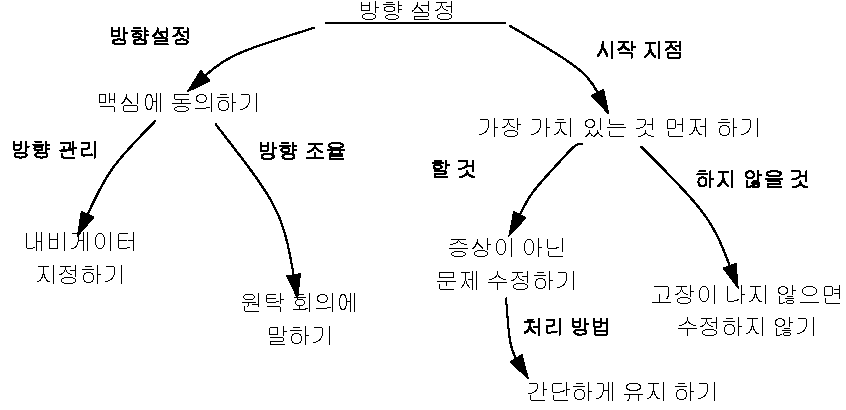
\includegraphics[width=\textwidth]{oldSettingDirectionMap.pdf}
\caption{리엔지니어링 프로젝트에서 방향을 설정하고 유지하기 위한 원칙과 지침}
\figlabel{SettingDirectionMap}
\end{center}
\end{figure}

%-----------------------------------------------------------------
\subsection*{Overview}

\charef{방향 설정}{SettingDirection}은 모든 개발 프로젝트에 적용할 수 있지만 리엔지니어링 작업과 특별한 관련성이 있는 패턴의 클러스터이다. 따라서 이를 설명하기 위해 문제(Problem), 해결책(Solution) 및 토론(Discussion)를 가지는 \emph{간결한 패턴 형식(streamlined pattern format)}을 선택했습니다.

리엔지니어링 팀 내에서 무엇이 문제이고 어떻게 달성할 수 있는지에 대한 공통된 이해를 확립하기 위해 \patref{맥심에 동의하기}{AgreeOnMaxims}를 작성해야 한다. 아키텍처 비전을 유지하기 위해 \patref{내비게이터 지정하기}{AppointANavigator}를 수행해야 한다. 모두가 \patref{라운드 테이블에 말하기}{SpeakToTheRoundTable}를 통해 프로젝트 상태에 대한 팀 인식을 유지해야 한다.

올바른 문제와 중요한 결정에 집중할 수 있도록 \patref{가장 가치 있는 것 먼저}{MostValuableFirst}를 사용하는 것이 현명하다. 이렇게 하면 \patref{사용자 참여시키기}{InvolveTheUsers} 및 \patref{자신감 만들기}{BuildConfidence}에 도움이 된다는 점에 참고하자. 래핑, 리팩터링 또는 재작성 여부를 결정하려면 \patref{증상이 아닌 문제 수정}{FixProblemsNotSymptoms}를 사용해야 한다. 변경을 위한 변경은 생산적이지 않으므로 \patref{고장이 나지 않으면 수정하지 않기}{IfItAintBrokeDontFixIt}를 사용하자. 새 시스템을 매우 유연하고 범용적으로 만들고 싶은 유혹이 있을 수 있지만, 거의 항상 \patref{단순함 유지하기}{KeepItSimple}을 사용하는 것이 더 좋다.

%=================================================================
%:PATTERN -- Agree on Maxims
\pattern{맥심에 동의하기}{AgreeOnMaxims}

\problem{팀에서 공통의 목적 의식(purpose)을 확립하려면 어떻게 해야 하는가?}

\solution{프로젝트의 핵심 우선순위를 정하고 팀이 궤도에 오르는 데 도움이 될 지침 원칙을 파악하자.}

\discussion
모든 리엔지니어링 프로젝트는 상충되는 수많은 이해관계에 대처해야 한다. 경영진은 제품의 경쟁력을 개선하고 유지보수 비용을 줄임으로써 레거시를 보호하고자 한다. 사용자는 기존 업무 패턴을 방해하지 않으면서 향상된 기능을 원한다. 개발자와 유지 관리자는 업무가 더 단순해지기를 원한다. 팀원들은 새로운 시스템의 모습에 대해 각자의 아이디어를 가지고 있을 수 있다.

\index{골드버그, 아델}
\index{루빈, 케니}
\emph{우리의 \ind{비즈니스 모델}(business model)은 무엇인가?} 또는 \emph{누가 무엇을 책임지는가?}와 같은 근본적인 질문에 대한 명확한 이해가 없다면 이해관계가 상충되어 팀이 분열되고 목표를 달성하지 못할 위험이 있다. 맥심(Maxim)은 여러 방향으로 끌려가는 프로젝트를 이끄는 데 도움이 되는 행동 규칙이다. 골드버그와 루빈은 \cite{Gold95a}에서 \emph{``모두가 테스트와 디버깅에 책임이 있다''}, \emph{``처음부터 제대로 할 수는 없다''} 등 수많은 \ind{맥심}의 예를 제시한다.

이 장의 모든 패턴은 팀을 안내하고 궤도에 맞추기 위한 것이므로 패턴이라기보다는 맥심(maxim)\footnote{행동에 본보기가 될 내용을 담고 있는 짧은 격언-옮긴이}으로 읽을 수 있다. 예를 들어 \patref{가장 가치 있는 것을 먼저}{MostValuableFirst}와 같은 맥심은 팀이 기술적으로는 흥미롭지만 레거시 시스템을 보호하거나 가치를 더하지 않는 한계적인 측면에 리엔지니어링 노력을 낭비하지 않도록 하기 위한 것이다. \patref{맥심에 동의하기}{AgreeOnMaxims}는 그 자체가 격언이므로 팀이 언제 방향타가 없는지 감지하는 데 도움이 될 수 있다.

기억해야 할 핵심 사항은 맥심의 수명이 제한적일 수 있다는 점이다. 채택된 맥심의 유효성을 주기적으로 재평가하는 것이 중요하다. 잘못된 맥심에 동의하거나 올바른 맥심에 동의하지만 시기가 잘못되면 프로젝트가 완전히 궤도에서 벗어날 수 있다.

%=================================================================
%:PATTERN -- Appoint a Navigator
\pattern{내비게이터 지정하기}{AppointANavigator}

\problem{복잡한 프로젝트 진행 중에 아키텍처 비전을 어떻게 유지하는가?}

\solution{아키텍처 비전이 유지될 수 있도록 내비게이터 역할을 담당할 사람을 지정하자.}

\discussion
모든 시스템의 \ind{아키텍처}는 시간이 지남에 따라 새로운 요구 사항과 관련성이 떨어지면서 성능이 저하되는 경향이 있다. 리엔지니어링 프로젝트의 과제는 레거시 시스템을 몇 년 더 지속하고 발전시킬 수 있는 새로운 아키텍처 비전을 개발하는 것이다. 내비게이터가 없으면 기존 시스템의 설계와 아키텍처가 새 시스템에 스며들어 그대로 이어지게 된다.

새로운 아키텍처가 해결해야 할 가장 중요한 문제가 무엇인지 결정하고 리엔지니어링 프로젝트 초기에 이러한 측면을 테스트할 수 있도록 \patref{가장 가치 있는 것을 먼저}{MostValuableFirst}를 해결해야 한다.

건전한 아키텍처는 \patref{증상이 아닌 문제 수정}{FixProblemsNotSymptoms}에 도움이 된다.

앨런 오캘러핸은 내비게이터를 ``불꽃의 수호자(Keeper of the Flame)''라고 부르기도 한다 \cite{Ocal99a}.

%=================================================================
%:PATTERN -- Speak to the Round Table
\pattern{원탁 회의에 말하기}{SpeakToTheRoundTable}

\problem{팀 소통의 동기화를 어떻게 유지하는가?}

\solution{간단하고 정기적인 원탁 회의를 개최하자.}

\discussion
레거시 시스템에 대한 지식과 이해는 항상 분산되어 있으며 대개 숨겨져 있다. 리엔지니어링 팀도 고고학을 수행하고 있다. 레거시 시스템에서 추출된 정보는 이를 활용하기 위해 반드시 공유해야 하는 귀중한 자산이다.

누구도 \ind{회의(meeting)}를 할 시간이 없지만, 회의가 없으면 커뮤니케이션은 임시방편적이고 무작위로 이루어진다. 정기적이고 집중적인 원탁 회의는 팀원들이 현재 상황에 대한 정보를 공유할 수 있도록 하는 목표를 달성할 수 있다. 원탁 회의는 짧게 진행하되 모든 사람이 참여해야 한다. 간단한 접근 방식은 모든 사람이 지난 회의 이후 무엇을 했는지, 무엇을 배웠는지, 또는 어떤 문제가 발생했는지, 다음 회의까지 무엇을 할 계획인지 말하도록 하는 것이다.

원탁 회의는 적어도 일주일에 한 번, 많게는 매일 개최하는 것이 좋다.

회의록은 진행 상황을 기록하는 데 중요하지만 회의록을 작성하는 것은 귀찮은 일이 될 수 있다. 회의록을 간단하게 작성하려면 특정 기한(deadline)까지 수행해야 할 \emph{결정사항(decisions)} 및 \emph{조치사항(actions)}만 기록하자.

\index{벡, 켄트}
\index{파울러, 마틴}
벡과 파울러는 원탁 회의를 짧게 진행하는 방법으로 ``스탠드업 미팅(Stand Up Meetings)''(의자 없는 회의)을 추천한다 \cite{Beck01a}.

%=================================================================
%:PATTERN -- Most Valuable First
\pattern{가장 가치 있는 것 먼저 하기}{MostValuableFirst}

\problem{어떤 문제에 먼저 집중해야 할까?}

\solution{고객에게 가장 가치 있는 측면부터 작업을 시작하자.}

\discussion
레거시 시스템에는 수많은 문제가 있을 수 있으며, 그 중에는 중요한 문제도 있고 고객의 비즈니스에 전혀 중요하지 않은 문제도 있을 수 있다. 가장 중요한 부분에 먼저 집중하면 문제가 되는 올바른 문제를 파악할 가능성이 높아지며, 마이그레이션할 \ind{아키텍처} 또는 새 시스템에 어떤 종류의 유연성을 구축할지 등 가장 중요한 결정을 프로젝트 초기에 테스트할 수 있다.

고객에게 가치 있는 시스템 부분에 먼저 집중함으로써 여러분과 팀원, 고객이 프로젝트에 대해 최대한 헌신할 수 있게 한다. 또한 리엔지니어링 노력이 가치 있고 필요하다는 것을 입증하는 긍정적인 결과를 조기에 얻을 가능성이 높아진다.

그럼에도 불구하고 이 패턴을 적용하는 데는 여러 가지 어려움이 있다.

\emph{고객은 누구인가?}

\index{이해관계자}
\begin{bulletlist}
  \item 모든 레거시 시스템에는 많은 이해관계자가 있지만 그 중 단 하나만 고른다면 고객이다. 누가 결정권을 가져야 하는지 명확하게 이해한 경우에만 우선순위를 설정할 수 있다.
\end{bulletlist}

\emph{무엇이 가치 있는 일인지 어떻게 알 수 있을까?}

\begin{bulletlist}
  \item 고객에게 가장 가치 있는 측면이 무엇인지 정확히 평가하는 것은 어려울 수 있다. 한 회사에서 아키텍처를 바꾸고 싶어서 시스템을 모듈화할 수 있는지 평가해 달라고 요청한 적이 있다. 하지만 오랜 논의 끝에 실제로는 비즈니스 규칙을 더 명확하게 표현할 수 있는 시스템이 필요하다는 것, 즉 한 명의 프로그래머만 이해하는 위험을 줄이기 위해 신입 프로그래머라도 더 쉽게 이해할 수 있는 시스템을 원한다는 것이 밝혀졌었다.

  \item 고객의 비즈니스 모델을 이해하려고 노력하라. 이를 통해 시스템의 다양한 측면의 가치를 평가하는 방법을 알 수 있다. 비즈니스 모델과 직접 관련이 없는 모든 것은 순전히 기술적인 측면의 문제일 가능성이 높다. 

  \item 고객이 얻고자 하는  \emph{측정 가능한 목표}가 무엇인지 파악하라. 예를 들어 응답 시간 개선, 새로운 기능의 출시 시간 단축, 개별 고객의 요구에 더 쉽게 맞춤화 등 시스템의 일부 측면 또는 시스템의 진화에 대한 외형적 표현이어야 한다.

  \item 주요 목표가 주로 \emph{기존 자산을 보호하는 것}인지, 아니면 새로운 기능이나 기능의 측면에서 \emph{가치를 추가하는 것}인지 이해하려고 노력하라.

  \item 변경 로그를 살펴보고 시스템에서 시간상으로 가장 많은 변경 활동이 있었던 위치를 파악하라. 가장 가치 있는 산출물(artifact)는 대개 가장 많은 변경 요청을 받은 산출물이다(\patpgref{과거로부터 학습}{LearnFromThePast} 참조). 

  \item 고객이 우선순위를 설정할 의향이 없거나 설정할 수 없는 경우에는 \emphind{계획 세우기 게임}(Planning Game)을 수행하자\cite{Beck01a}. 모든 이해관계자로부터 요구사항을 수집하고 식별 가능한 각 작업에 필요한 노력에 대한 대략적인 추정치를 만든다. 초기 첫 번째 마일스톤에 대한 초기 노력 예산이 주어지면 고객에게 예산에 맞는 작업을 선택하도록 요청한다. 각 반복(iteration)마다 이 플래닝 게임 적용을 실천한다.

  \item \emph{인식 변화(changing perceptions)}에 주의하라. 처음에는 고객이 문제 자체보다는 레거시 시스템에서 나타나는 특정 증상에 주목할 수 있다(\patpgref{증상이 아닌 문제 수정}{FixProblemsNotSymptoms} 참조). 
\end{bulletlist}

\emph{기대치가 너무 높아질 위험이 있지 않는가?}

\begin{bulletlist}
  \item 좋은 초기 결과를 제공하지 못하면 많은 것을 배울 수 있지만 신뢰도를 잃을 위험이 있다. 따라서 고객에게 가치를 제공할 뿐만 아니라 성공 가능성도 높은 초기 작업을 신중하게 선택하는 것이 중요하다. 따라서 초기 작업의 노력을 추정할 때 세심한 주의를 기울이자.

  \item 성공의 열쇠는 작고 빈번한 반복(iteration)을 계획하는 것이다. 고객이 파악한 초기 작업이 너무 커서 단기간(예: 2주)에 초기 결과를 보여줄 수 없다면 더 짧은 반복으로 해결할 수 있는 작은 하위 작업으로 세분화하자. 첫 단계에 성공하면 기대치가 높아지겠지만, 단계가 작아도 나쁘지 않다.
\end{bulletlist}

\emph{가장 가치 있는 부분이 쥐의 둥지(rat's nest)라면 어떨까?}

\begin{bulletlist}
  \item 안타깝게도 레거시 시스템을 리엔지니어링하는 것은 정상적이고 주기적인 혁신 프로세스가 아니라 절박한 상황에서 이루어지는 경우가 많다. 시스템에서 가장 중요한 부분이 가장 복잡하고 난공불락이며 수정과 디버깅이 어려운 부분일 수도 있다. 

  \item 높은 변경률(high changes rates)은 소프트웨어 결함이 많다는 신호일 수도 있다. 소프트웨어 결함의 80\%는 일반적으로 코드의 5\%에서 발생하므로 ``최악을 먼저 고친다''는 전략은 시스템에서 가장 심각한 문제의 원인을 제거함으로써 큰 성과를 거둘 수 있다 \cite{Davi95a}. 그럼에도 불구하고 상당한 위험이 따른다.

	\begin{bulletlist}
    \item 	조기에 긍정적인 결과를 입증하기 어려울 수 있다.
  
    \item 	정보가 거의 없는 상태에서 시스템의 가장 복잡한 부분을 다룰 수 있다.

    \item 	실패할 가능성이 높다.
	\end{bulletlist}

  \item 문제가 있는 구성 요소를 래핑할지, 리팩터링할지 또는 다시 작성할지 여부를 \patref{증상이 아닌 문제 수정}{FixProblemsNotSymptoms}를 확인하여 결정한다.

\end{bulletlist}

시스템에서 작업할 가장 중요한 부분이 무엇인지 결정한 후에는 리엔지니어링 노력에 \patpgref{사용자 참여시키기}{InvolveTheUsers}를 수행하여 \patpgref{신뢰 구축하기}{BuildConfidence}을 수행해야 한다. \patpgref{시스템 점진적 마이그레이션하기}{MigrateSystemsIncrementally}을 사용하면 사용자가 리엔지니어링된 시스템을 사용하면서 지속적인 피드백을 제공할 수 있다.

%=================================================================
%:PATTERN -- Fix Problems, Not Symptoms
\pattern{증상이 아닌 문제 수정하기}{FixProblemsNotSymptoms}

\problem{보고된 모든 문제를 어떻게 해결할 수 있을까?}

\solution{이해관계자의 요청이 아닌 문제의 원인을 해결하자.}

\discussion
이것은 매우 일반적인 원칙이지만 리엔지니어링과 특히 관련이 있다. \ind{이해관계자}\emph{(stakeholder)}마다 시스템에 대한 관점이 다르고 시스템의 일부만 볼 수도 있다. 그들이 고치기를 원하는 문제는 시스템의 더 깊은 문제를 드러내는 것일 수도 있다. 예를 들어 특정 사용자 작업에 대한 즉각적인 피드백을 받지 못하는 것은 데이터 흐름 아키텍처의 결과일 수 있다. 해결 방법을 구현하면 문제가 악화되어 더 많은 해결 방법이 필요할 수 있다. 이것이 진짜 문제라면 적절한 아키텍처로 마이그레이션해야 한다.

리엔지니어링 작업 중 흔히 발생하는 어려움은 레거시 컴포넌트를 래핑할지, 리팩터링할지, 다시 작성할지 결정하는 것이다. \patref{가장 가치 있는 것 먼저 하기}{MostValuableFirst}는 시스템의 문제에 어떤 우선순위를 부여할지 결정하는 데 도움이 되며, 어떤 문제가 중요한 경로에 있는지를 알려준다. \patref{증상이 아닌 문제 수정하기}{FixProblemsNotSymptoms}는 문제의 현상이 아닌 문제의 원인에 집중하도록 한다. 예를 들자면 다음과 같은 것들이 있다.

\begin{bulletlist}
  \item 레거시 컴포넌트의 코드가 기본적으로 안정적이고 문제가 주로 클라이언트 변경에서 발생하는 경우, 코드가 아무리 엉망이라도 구현이 아니라 레거시 컴포넌트에 대한 인터페이스에 문제가 있을 가능성이 높다. 이러한 경우 \patpgref{올바른 인터페이스 제공하기}{PresentTheRightInterface}를 적용하여 인터페이스만 수정하는 것을 고려해야 한다.

  \item 레거시 컴포넌트에 결함이 거의 없지만 시스템 변경에 큰 병목 현상이 발생하는 경우 향후 변경의 영향을 제한하기 위해 리팩터링해야 할 수도 있다. 보다 깔끔한 디자인으로 마이그레이션하기 위해 \patpgref {신 클래스 분할하기}{SplitUpGodClass}를 적용하는 것을 고려할 수 있다.

  \item 레거시 컴포넌트에 많은 결함이 있는 경우, 레거시 데이터를 새 구현으로 마이그레이션하기 위한 전략으로 \patpgref{새로운 마을로 다리 만들기}{MakeABridgeToTheNewTown}을 적용하는 것을 고려하자.
\end{bulletlist}

이 패턴은 \patref{고장이 나지 않으면 수정하지 않기}{IfItAintBrokeDontFixIt}과 충돌하는 것처럼 보일 수 있지만 실제로는 그렇지 않다. 실제로 '깨지지 않은' 것은 문제의 원인이 될 수 없다. 예를 들어 래핑은 해결 방법처럼 보일 수 있지만 실제 문제가 레거시 컴포넌트에 대한 인터페이스에만 있는 경우 올바른 해결책이 될 수 있다.

%=================================================================
%:PATTERN -- If It Ain't Broke, Don't Fix It
\pattern{고장이 나지 않으면 수정하지 않기}{IfItAintBrokeDontFixIt}

\problem{레거시 시스템에서 어떤 부분을 리엔지니어링하고 어떤 부분을 그대로 둬야 할까?}

\solution{``고장난'' 부분, 즉 계획된 변경에 더 이상 적용할 수 없는 부분만 수정하자.}

\discussion
변화를 위한 변화가 반드시 좋은 것만은 아니다. 레거시 시스템에는 보기 흉할 수 있지만 잘 작동하고 유지 관리에 큰 부담이 되지 않는 부분이 있을 수 있다. 이러한 구성 요소를 분리하고 포장할 수 있다면 교체할 필요가 없을 수도 있다.

무언가를 ``수정''할 때마다 시스템의 다른 무언가가 손상될 위험도 있다. 또한 사소한 문제에 귀중한 시간과 노력을 낭비할 위험도 있다.

리엔지니어링 프로젝트에서 ``고장난'' 부분은 레거시를 위험에 빠뜨리는 부분이다.
\begin{bulletlist}
  \item 새로운 요구 사항을 충족하기 위해 자주 조정해야 하지만 높은 복잡성과 디자인 드리프트(design drift)\footnote{설계와 구현의 차이-옮긴이}로 인해 수정하기 어려운 컴포넌트(component).
  
  \item 중요하지만 전통적으로 많은 결함을 포함하는 컴포넌트.
\end{bulletlist}

안정적이고 레거시 시스템의 미래를 위협하지 않는 소프트웨어 산출물은 코드가 어떤 상태에 있든 ``고장난'' 것이 아니므로 다시 엔지니어링할 필요가 없다.

%=================================================================
%:PATTERN -- Keep It Simple
\pattern{간단하게 유지 하기}{KeepItSimple}

\problem{새 시스템에 얼마나 많은 유연성을 구축해야 할까?}

\solution{더 일반적이고 복잡한 솔루션보다 적절하고 간단한 솔루션이 더 낮다.}

\discussion
이것은 리엔지니어링에 특별한 의미를 갖는 또 다른 일반적인 원칙이다. 우리는 실제로 얼마나 많은 일반성과 유연성이 필요한지 추측하는 데 서툴다. 많은 소프트웨어 시스템은 생각할 수 있는 모든 기능이 추가되면서 비대해진다.

유연성(flexibility)은 양날의 검입니다. 리엔지니어링의 중요한 목표는 미래의 변화를 수용하는 것이다. 하지만 지나친 유연성은 새로운 시스템을 너무 복잡하게 만들어 오히려 미래의 변화를 방해할 수 있다.

어떤 사람들은 ``재사용을 위한 계획(plan for reuse)''이 필요하므로 누군가에게 유용할 수 있는 모든 소프트웨어 개체가 가능한 한 많은 노브와 버튼으로 가능한 가장 일반적인 방식으로 프로그래밍되도록 추가적인 노력을 기울여야 한다고 주장한다. 하지만 누가 어떤 용도로 어떤 것을 사용할지 예측하는 것은 거의 불가능하기 때문에 이런 방식은 거의 효과가 없다. 최종 사용자 소프트웨어도 마찬가지이다.

\seeindex{XP}{익스트림 프로그래밍}
``\ind{일할 수 있는 가장 간단한 것을 하라}''는 \ind{익스트림 프로그래밍}의 맥심이다. \cite{Beck00a}의 맥심으로, 모든 리엔지니어링 노력에 적용된다. 이 전략은 사용자가 평가하고 대응할 수 있는 간단한 변경 사항을 신속하게 도입하도록 장려하기 때문에 \patpgref{사용자 참여 시키기}{InvolveTheUsers} 및 \patpgref{신뢰 구축 하기}{BuildConfidence}을 강화한다.

복잡한 작업을 수행하면 (실제로 필요한 것이 무엇인지) 잘못 추측할 수 있고 수정하기가 더 어려워진다. 일을 단순하게 유지하면 더 빨리 끝내고, 더 빨리 피드백을 받고, 더 쉽게 오류를 복구할 수 있다. 그런 다음 다음 단계로 넘어갈 수 있다.

%=============================================================
\ifx\wholebook\relax\else
   \bibliographystyle{alpha}
   \bibliography{scg}
   \end{document}
\fi
%=============================================================
